 \documentclass[svgnames]{article}
\usepackage[utf8]{inputenc}
\usepackage{amsmath}
\usepackage{amssymb}
\usepackage{mathrsfs}
\usepackage{mathtools}
\newtheorem{mydef}{Given}
\newtheorem{mytheorem}{Theorem}
\usepackage{enumitem}
\usepackage{venndiagram}
\usepackage{smartdiagram}
\usepackage{caption}
\usepackage{subcaption}
%\usepackage[framed,numbered,autolinebreaks,useliterate]{mcode}
\usepackage{pgfplots}
%\usepackage{tkiz}



\usepackage{listings}
\usepackage{color}

\definecolor{dkgreen}{rgb}{0,0.6,0}
\definecolor{gray}{rgb}{0.5,0.5,0.5}
\definecolor{mauve}{rgb}{0.58,0,0.82}

\lstset{frame=tb,
  language=Java,
  aboveskip=3mm,
  belowskip=3mm,
  showstringspaces=false,
  columns=flexible,
  basicstyle={\small\ttfamily},
  numbers=none,
  numberstyle=\tiny\color{gray},
  keywordstyle=\color{blue},
  commentstyle=\color{dkgreen},
  stringstyle=\color{mauve},
  breaklines=true,
  breakatwhitespace=true,
  tabsize=3
}
\usepackage{graphicx}
\graphicspath{ {./images/} }
%\renewcommand{\theenumi}{\Alph{enumi}}
\newenvironment{amatrix}[1]{%
  \left(\begin{array}{@{}*{#1}{c}|c@{}}
}{%
  \end{array}\right)
}

\newenvironment{tolerant}[1]{%
  \par\tolerance=#1\relax
}{%
  \par
}


\title{Statistical methods: Homework 6}
\author{Cameron McIntyre}
\date{October 2018}

\begin{document}

\maketitle

\section{4.2.4}
A chromosome mutation linked with colorblindness is known to occur, on the average, once in every ten thousand births.

\textbf{Answer:}
\begin{enumerate}[label=(\alph*)]

\item Approximate the probability that exactly three of the next twenty thousand babies born will have the mutation.

$\lambda=20000*\frac{1}{10000}=2$
$$P(X=3)=\frac{1}{e^{\lambda}}\frac{\lambda^n}{n!}=\frac{1}{e^{2}}\frac{(2)^3}{3!}=.1804$$

\item  How many babies out of the next twenty thousand would have to be born with the mutation to convince you that the one in ten thousand estimate is too low.

$$P(X > n) = 1 - P(X \leq n-1) =1- \sum^{0}_{n-1}P(x=k) = 1- \sum^{0}_{n-1}\frac{1}{e^{2}}\frac{(2)^n}{n!}$$

We go to r to get some values:
\begin{lstlisting}
1 -cumsum(dpois(c(0:10),2))
\end{lstlisting}
$$ P(X\geq 1) =  0.864664 $$
$$ P(X\geq 2) =  0.5939942 $$
$$ P(X\geq 3) =  0.3233236 $$
$$ P(X\geq 4) =  0.1428765 $$
$$ P(X\geq 5) =  0.05265302 $$
$$ P(X\geq 6) =  0.01656361 $$
$$ P(X\geq 7) =  0.00453380 $$ 
$$ P(X\geq 8) =  0.00109671$$
$$ P(X\geq 9) =  0.00023744 $$
$$ P(X\geq 10) =  0.0000464 $$
$$ P(X\geq 11) =  0.0000083$$

If there are 3 or more births with the mutation in 20000. then I would say the estimate needs to be revised because that should only happen 32\% of the time. Also 60\% of the time there will be 2 children with the defect. This is more than half the time. This also makes me think the estimate should be revised. 
\end{enumerate}


\section{4.2.12}

Midwestern Skies books ten commuter flights each week. Passenger totals are much the same from week to week, as are the numbers of pieces of luggage that are checked. Listed in the following table are the numbers of bags that were lost during each of the first forty weeks in 2009. Do these figures support the presumption that the number of bags lost by Midwestern during a typical week is a Poisson random variable?


\textbf{Answer:}
The average number of bags lost in a given week is 1.525 bags/week.

Using R we calculate probabilities
\begin{lstlisting}
> dpois(c(0:10),1.525)
[1] 2.176211e-01 3.318721e-01 2.530525e-01 1.286350e-01 4.904210e-02
[6] 1.495784e-02 3.801784e-03 8.282459e-04 1.578844e-04 2.675263e-05
[11] 4.079776e-06
> sum(dpois(c(0:10),1.525))
[1] 0.9999994
\end{lstlisting}
 $$ P(X = 0) = .2176211 \ versus\  22.5\% \ from \ the \ data$$
 $$ P(X = 1) = .3318721 \ versus\  32.5\% \ from \ the \ data$$
 $$ P(X = 2) = .2530525 \ versus\   25\% \ from \ the \ data$$
 $$ P(X = 3) = .1286350 \ versus\  12.5\% \ from \ the \ data$$
  $$ P(X = 4) = .04904210 \ versus\  5\% \ from \ the \ data$$
  $$ P(X = 5) = .01495784 $$
   $$ P(X = 6) =  .003801784$$
 $$ P(X = 7) = .0008282459 $$
  $$ P(X = 8) = .0001578844 $$
   $$ P(X = 9) = .00002675263$$
 $$ P(X = 10) =  .000004079776$$

The data from the airline is definitely modelled well by a poisson distribution.

\section{4.2.28}
Fifty spotlights have just been installed in an out-door security system. According to the manufacturer?s specifications, these particular lights are expected to burn out at the rate of 1.1 per one hundred hours. What is the expected number of bulbs that will fail to last for at least seventy-five hours?
\newline
\newline
\textbf{Answer:}

For this scenario $\lambda=1.1 \frac{bulbs}{100\ hours}$
Therefore the probability of a single bulb lasting less than 75 hours is $$P(H<75)=(1-e^{-1.1\cdot \frac{75}{100}})=1-e^{-1.1\cdot .75}=.5617$$
$$50\cdot .5617=28.09$$

So, we can estimate that out of the 50 new lights, 28 will have failed.  

\section{4.3.2}
\begin{enumerate}[label=(\alph*)]
\item Let $0<a<b$. Which number is larger?

$$\int^{b}_{a}\frac{1}{\sqrt{2\pi}}e^{-\frac{z^2}{2}} \ or\  \int^{-a}_{-b}\frac{1}{\sqrt{2\pi}}e^{-\frac{z^2}{2}}$$

\textbf{Answer:}
The two quantities are equal. We rely on the symmetry about 0 of the normal distribution to show this.

Consider only $f(z) = e^{-\frac{z^2}{2}}$. For any number $a$ we can show that $f(-a)=f(a)$.

$$f(-a) = e^{-\frac{(-a)^2}{2}} = e^{-\frac{(-1)^2a^2}{2}} = e^{-\frac{(1\cdot a^2)}{2}} = f(a) $$

Therefore,

\[ \int^{b}_{a}\frac{1}{\sqrt{2\pi}}e^{-\frac{z^2}{2}}=P(a<Z<b) = 1 - (P(Z<a) + P(Z > b))\]
\[= 1 - (P(Z> -a) + P(Z < - b)) (by \ symmetry) \]
\[= P(-b < Z < -a) \]
\[= \int^{-a}_{-b}\frac{1}{\sqrt{2\pi}}e^{-\frac{z^2}{2}} \]

\item Let $a>0$. Which number is larger?

$$\int^{a+1}_{a}\frac{1}{\sqrt{2\pi}}e^{-\frac{z^2}{2}} \ or\  \int^{a+\frac{1}{2}}_{a-\frac{1}{2}}\frac{1}{\sqrt{2\pi}}e^{-\frac{z^2}{2}}$$

\textbf{Answer:}

 $\int^{a+\frac{1}{2}}_{a-\frac{1}{2}}\frac{1}{\sqrt{2\pi}}e^{-\frac{z^2}{2}}$ is the larger quantity.
 
Consider only $f(z) = e^{-\frac{z^2}{2}}$

Then, $f'(z)=-z e^{-\frac{z^2}{2}}$, Clearly $f'(z)<0 \ \forall \  z >0 $.

Now( $a+1-a )=1$ and also $(a+\frac{1}{2} - (a-\frac{1}{2}))=1$ Therefore the integrals are over the same length domain.

But, $f(a+\epsilon)<f(a)$ because $f'(a)<0$. Therefore the normal function is always less over the interval $[a, a+1]$, compared to $[a-\frac{1}{2}, a+\frac{1}{2}]$. 

So we can then conclude
$$\int^{a+1}_{a}\frac{1}{\sqrt{2\pi}}e^{-\frac{z^2}{2}} <  \int^{a+\frac{1}{2}}_{a-\frac{1}{2}}\frac{1}{\sqrt{2\pi}}e^{-\frac{z^2}{2}}$$

\end{enumerate}

\section{4.3.14}
A sell-out crowd of 42,200 is expected at Cleveland\textsc{\char13}s Jacobs Field for next Tuesday\textsc{\char13}s game against the Baltimore Orioles, the last before a long road trip. The ballpark\textsc{\char13}s concession manager is trying to decide how much food to have on hand. Looking at records from games played earlier in the season, she knows that, on the average, 38$\%$ of all those in attendance will buy a hot dog. How large an order should she place if she wants to have no more that a 20\% chance of demand exceeding supply?

\textbf{Answer:}

Our estimate for $\mu$ is $\mu=np=42200*.38=16036$.

Our estimate for $\sigma$ is $\sigma=\sqrt{np(1-p)}=42200\cdot.38\cdot.62=99.7112$

We need to find the number of hot dogs (\textbf{X}) such that the probability of running out does not exceed 20\textsc{\char13}s.

Using R we find the z score for 80\textsc{\char13}s.
\begin{lstlisting}
> qnorm(.8)
[1] 0.8416212
\end{lstlisting}

We can get our estimate for \textbf{X} in the following way.
$$\frac{X-\mu}{\sigma}=\frac{X-16036}{99.711}=0.8416212 $$
$$X=16,120$$

Therefore the person running the hot dog stand should order 16,120 hotdogs, if they are aiming to have an 80\% chance they don't run out (equivalently 20\% chance they do run out).

\section{4.3.18}
 Suppose $X_1,X_2,X_3$and $X_4$ are independent Poisson random variables, each with parameter ? = 3. Let $S = X_1 +X_2 +X_3 +X_4$.
\begin{enumerate}[label=(\alph*)]
\item
Use the Central Limit Theorem to approximate the probability that $13 \leq S \leq 14$. 
We get our approximations $\mu_s= 4*3$ and $\sigma_s=\sqrt{4*3}=3.46$

$$z(S)=\frac{S-mu_s}{\sigma_s}$$

And $z(14)$=.58, similarly $z(13)=.29$

Now Using the tables $P(.29<Z<.48)=.1050$


\item Calculate the exact probability that $13 \leq S \leq 14$. 

We can add Poisson Variable together. So $\mu=3+3+3+3=12$ and 

$$\sum_{i=13}^{14}e^{-12}\frac{12^i}{i!}=e^{-12}\frac{12^{13}}{13!}+e^{-12}\frac{12^{14}}{14!}=+1056+0905=.1961$$

We could eliminate some of the difference by adding in the continuity correction from the lectures. 

\end{enumerate}

\section{4.3.22}
 A large computer chip manufacturing plant under construction in Westbank is expected to result in an additional fourteen hundred children in the county?s public school system once the permanent workforce arrives. Any child with an IQ under 80 or over 135 will require individualized instruction that will cost the city an additional \$1750 per year. How much money should Westbank anticipate spending next year to meet the needs of its new special ed students? Assume that IQ scores are normally distributed with a mean ($\mu$) of 100 and a standard deviation ($\sigma$) of 16.

\textbf{Answer:}

We can assume $IQ \sim N(100,16)$. We need to estimate the number of children with and IQ $>135$ and others with and IQ $< 80$.

$$P(X>135) = P(\frac{X - \mu}{\sigma}> 2.1875)=P(z>  2.1875)=0.01435302$$
$$P(X<85) = P(\frac{X - \mu}{\sigma}>-1.25)=P(z> -1.25)=0.1056498$$

From this we can estimate that $0.01435302\cdot 1400=20.09$ Kids will be on the high end and  $0.1056498\cdot 1400=147.909$ will be on the low end. That would suggest they will be spending approximately $(147.909 + 20.01)*1750=293,858.2$\$ on special education.


\section{4.4.6}
Suppose three fair dice are tossed repeatedly. Let the random variable X denote the roll on which a sum of 4 appears for the first time. Use the expression for $FX(t)$ given in Question 4.4.5 to evaluate $P(65 \leq X \leq 75)$.

\textbf{Answer:}

We have to figure out the probability $p$ of the successful event, namely, the sum being equal to 4. This can happen 3 possible ways. Therefore $p=\frac{6}{216}$ 

Our expression
$$F(X(t)) = P(X \leq t) = 1 - (1 - p)^t $$

Can then be used in the following way:

\[P(65\leq X \leq75)=P(X\leq75)-P(X\leq64) = \Big(1 - (1 -\frac{6}{216})^{75}\Big) -\Big(1 - (1 -\frac{6}{216})^{64}\Big)\]
\[=0.8791029-0.8351857=0.04391719\]


\section{4.4.10}
Suppose that the random variables $X_1$ and $X_2$ have mgfs $M_{X_1}(t) =\frac{\frac{1}{2} e^t}{1-(1-\frac{1}{2})e^t}$ and $M_{X_2}(t) = \frac{\frac{1}{4}e^t}{1-(1-\frac{1}{4})e^t}$, respectively. Let $X = X_1 +X_2$.Does X have a geometric distribution? Assume that X1 and X2 are independent.
\newline
\newline
\textbf{Answer:}
Using Theorem 3.12.3 , if $X=X_1+X_2+...+X_n$, and each of the $X_i$ are independent with MGFs $M_{X_{i}}(t)$. Then, $M_{X}(t)=\Pi_{1}^{n}M_{X_i}(t)$.
\newline
\newline
We also know the mgf of the geometric distribution $\frac{pe^t}{1-(1-p)e^t} $. Therefore $X_1\sim geom(\frac{1}{2})$ and $X_2\sim geom(\frac{1}{4})$.
\newline
\newline
The product of their MGFs is:
$$ M_{X}(t)=M_{X_1}(t)\cdot M_{X_2}(t)=\frac{\frac{1}{2} e^t}{1-(1-\frac{1}{2})e^t}\cdot \frac{\frac{1}{4}e^t}{1-(1-\frac{1}{4})e^t}= \frac{\frac{1}{8}e^{2t}}{1-e^t(\frac{3}{4}e^t-\frac{1}{4})}$$

This new MGF looks nothing like a geometric MGF. Therefor $X=X_1+X_2$ is not geometrically distributed

\section{4.5.5}
 For a negative binomial random variable whose pdf is given by Equation 4.5.1, find $E(X)$ directly by evaluating $\sum^{\infty}_{r}\binom{k-1}{r-1}p^{r}(1-p)^{k-r}$.(Hint: Reduce the sum to one
involving negative binomial probabilities with parameters r + 1 and p.)
\newline
\newline
\textbf{Answer:}
$$E(K)=\sum^{\infty}_{k=r}k\binom{k-1}{r-1}p^{r}(1-p)^{k-r}=\sum^{\infty}_{k=r}\frac{r}{p}\frac{k*(k-1)!}{(k-r)!r(r-1)!}p^{r+1}(1-p)^{k-r}$$

$$\frac{r}{p}\sum^{\infty}_{k=r}\binom{k}{r}p^{r+1}(1-p)^{k-r}=\frac{r}{p}*1=\frac{r}{p}$$

\section{4.6.2}
A service contact on a new university computer system provides twenty-four free repair calls from a technician. Suppose the technician is required, on the average, three times a month. What is the average time it will take for the service contract to be fulfilled?
\newline
\newline
\textbf{Answer:}

Using the expected value property of the gamma distribution the average time a contract will take to be fufilled is $\frac{r}{\lambda}=\frac{24}{3}=8$ months.

\section{4.6.6}
Prove that $\Gamma(\frac{1}{2})=\sqrt{\pi}$. (Hint: Consider $E(Z^2)$, where Z is a standard normal random variable.)
\newline
\newline
\textbf{Answer:}
This question requires a bit of extra machinery. Our strategy is to take the gamma function, assume it has a finite interval, make a variable substitution, then find the square of that integral, transform into polar co-ordinates, integrate over the new bounds and then hope that it equals $\sqrt{\pi}$ - which it does because its a well established result.
\newline
So,

$$\Gamma(\alpha)=\int_{0}^{\infty}x^{\alpha-1}e^{-x}dx$$
We let $\alpha=\frac{1}{2}$ substitute $x=u^2$, (then $dx = 2udu$) and we get,
$$\Gamma(\frac{1}{2})=\int_{0}^{\infty}u^{2*\frac{1}{2}}e^{-u^2}2udu=2\int_{0}^{\infty}e^{-u^2}du$$

Lets assume that this integral has value a finite value. Then the product of two identical integrals will have a finite value.
$$\Big(\Gamma(\frac{1}{2})\Big)^2=2\int_{0}^{\infty}e^{-u^2}du \cdot 2\int_{0}^{\infty}e^{-v^2}dv = 4\int_{0}^{\infty}\int_{0}^{\infty}e^{-(u^2+v^2)}dudv $$

We now change to polar co-ordinates:
$$\Big(\Gamma(\frac{1}{2})\Big)^2 =4 \int_{0}^{\infty}\int_{0}^{\frac{\pi}{2}}e^{-r^2}rd\theta dr $$

Substitute $z=r^2$, then $dz = 2rdr$
$$\Big(\Gamma(\frac{1}{2})\Big)^2 = 2\int_{0}^{\frac{\pi}{2}}\int_{0}^{\infty}e^{-z}dzd\theta=2\int_{0}^{\frac{\pi}{2}}[-e^{-z}]\Big|^{z=\infty}_{0}=2\int_{0}^{\frac{\pi}{2}}-[0-1] d\theta=2[\frac{\pi}{2}-0]=\pi$$

So,
$$\Big(\Gamma(\frac{1}{2})\Big)^2 = \pi. \leftrightarrow \Gamma(\frac{1}{2})=\sqrt{\pi}$$


\section{4.6.9}
Differentiate the gamma moment-generating function to verify the formulas for E(Y)and Var(Y) given in Theorem 4.6.3.
\newline
\newline
\textbf{Answer:}

Gamma Moment generating function:
$$ M_Y(t) = (1 - \frac{t}{\lambda})^{-r}$$

Finding the expectation, we differentiate wrt t and evaluate at t=0.
$$E[Y] = M_Y'(t)\Big|_{t=0} = -r(1 - \frac{t}{\lambda})^{-r-1}*\frac{-1}{\lambda}\Big|_{t=0}=\frac{r}{\lambda}(1-\frac{t}{\lambda})^{r-1}\Big|_{t=0}=\frac{r}{\lambda}$$

So as expected $E[Y] =\frac{r}{\lambda}$.
\newline
\newline
For $E[Y^2]$ we find $M_Y''(t)\Big|_{t=0}$

$$\frac{d}{dt}\frac{r}{\lambda}(1-\frac{t}{\lambda})^{-(r+1)}\Big|_{t=0}=\frac{r(r+1)}{\lambda}(1-\frac{t}{\lambda})^{-(r+1)}\frac{-1}{\lambda}\Big|_{t=0}=\frac{r(r+1)}{\lambda^2}$$
\newline
\newline
Then the variance is $Var[Y]=E[Y^2]-(E[Y])^2$

$$Var[Y]=E[Y^2]-(E[Y])^2=\frac{r(r+1)}{\lambda^2}-\frac{r^2}{\lambda^2}=\frac{r}{\lambda^2}$$



\textbf{PROGRAMMING ASSIGNMENT}

\textbf{RESULTANT GRAPH FOLLOWS LINE Y=X, SUGGESTING THE SUM OF 3 POISSON VARIABLES IS POISSON DISTRIBUTED, LINE Y=X SHOWN IN BLUE.}

\textbf{Part A}
\begin{lstlisting}
poi1 <- qpois(runif(1000),2)
poi2 <- qpois(runif(1000),2)
poi3 <- qpois(runif(1000),2)

poi_combined = poi1 + poi2 + poi3

poi_total <- qpois(runif(1000),6)

poi_combined = sort(poi_combined)

poi_total = sort(poi_total)

plot(poi_combined,poi_total)
\end{lstlisting}

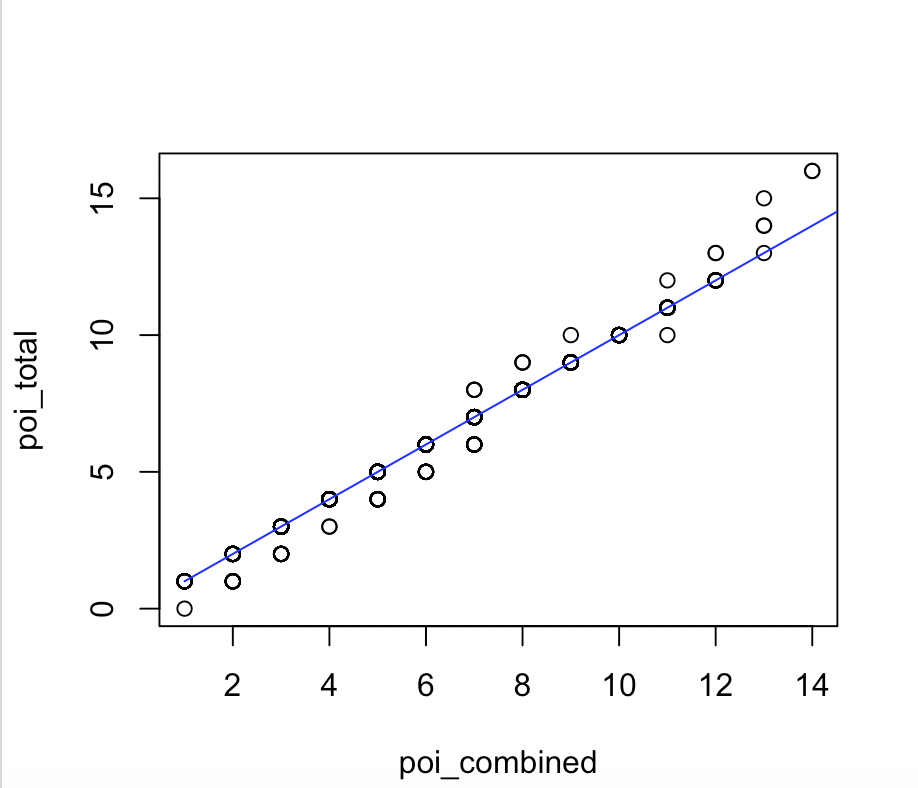
\includegraphics[scale=.65]{PoissonSUM}


\textbf{Part B}

\textbf{WE KNOW THAT THE SUM OF THE 3 EXPONENTIAL VARIABLES ARE DISTRIBUTED AS GAMMA WITH PARAMETER LAMBDA = $\frac{1}{2}$ AND SHAPE PARAMETER 3. WE SHOW THIS GRAPHICALLY BY SUMMING 3 EXPONENTIAL RANDOM VARIABLES AND GRAPHING THEM AGAINST A GAMMA RANDOM VARIABLE. LINE Y=X SHOWN IN BLUE}

\begin{lstlisting}
exp1 <- qexp(runif(1000),.5)
exp2 <- qexp(runif(1000),.5)
exp3 <- qexp(runif(1000),.5)

exp_combined = exp1 + exp2 + exp3

exp_total <- qgamma(runif(1000),shape=3, rate =.5)

exp_combined = sort(exp_combined)

exp_total = sort(exp_total)

plot(exp_combined[51:950],exp_total[51:950], col= 'green')
lines(x= c(1:12),y = c(1:12),col='blue', add= T)
plot(exp_combined[51:950],exp_total[51:950])
\end{lstlisting}
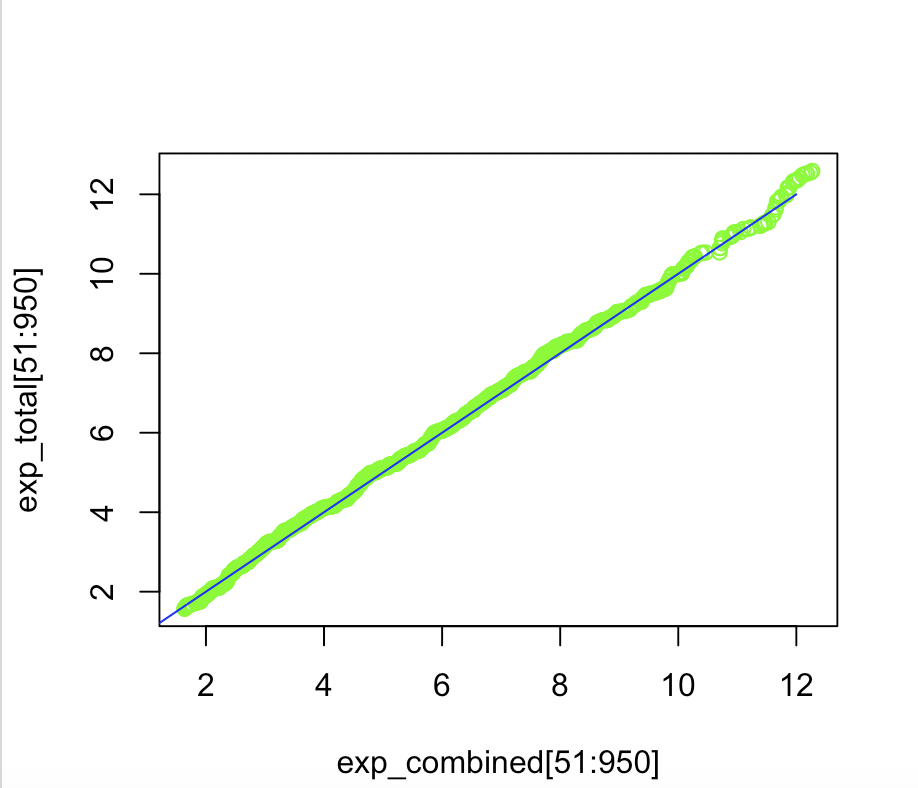
\includegraphics[scale=.65]{Exponentialsum}
\end{document}